% !TEX root = ../thesis.tex

\chapter{Meranie kvantových obvodov}

Jediným spôsobom ako zistiť skutočný stav kvantového obvodu je meraním.
Merať možno všetky bity súčasne ako aj jednotlivé kvantové bity samostatne.

\section{Princíp merania kvantových obvodov}

Kvantový bit môže existovať v nekonečnom množstve stavov. Meranie si môžme 
predstaviť ako prevod stavov kvantových bitov do stavu klasického digitálneho
systému \cite{Nie10}. Pre príklad môžeme reprezentovať kvantový stav 
\(\alpha\ket{0} + \beta\ket{1}\) pomocou nulového a excitovaného stavu atómu.
Skutočný kvantový počítač by tak mohol merať tieto stavy \cite{Sim97}
. Pri meraní by 
daný atóm skolaboval do jedného zo stavov \(\ket{0}\) alebo \(\ket{1}\).
Pre kolabovanie samozrejme rovnako platí to, že do jednotlivých stavov by
sa atóm dostal s pravdepodobnosťami \(|\alpha|^2\) respektíve \(|\beta|^2\).


Pri každom fyzikálnom meraní nastáva určitá nepresnosť merania. Takisto 
pri meraní môže dokonca nastať zničenie obvodu. To vyplýva z toho, že pri
skolabovanom kvantovom bite nastáva zmena fyzikálnych vlastností daného bitu. 

\section{Fiktívne meranie}

Našim cieľom je navrhnúť pravdepodobnostný model, ktorý by umožnil merať
stavy kvantových obvodov aj bez kolabovania jednotlivých kvantových bitov.

\subsection{Experiment 1}
Navrhnime kvantový obvod s dvoma bitmi. Označme ich \(\ket{\psi_0}\) a 
\(\ket{\psi_1}\). V prvom kroku aplikujeme Hadamardovo hradlo na bit 
\(\ket{\psi_0}\). Nasledovať budú dve \(CNOT\) hradlá, s opačnými kontrólnymi 
a cieľovými bitmi. V IBM QX je tento obvod reprezentovaný ako 
\begin{code}
qreg q[2];
creg c[2];

h q[0];
cx q[0],q[1];
cx q[1],q[0];
\end{code}
Jeho grafické zobrazenie je na obrázku \ref{expr1_circuit}, aj s označenými
časovými úsekmi, v ktorých bude meraný stav systému. 

\begin{figure} 
	\centering 
	\includegraphics[width=.6\textwidth]{figures/expr1_circuit.png} 
	\caption{Obvod experimentu 1 s označenými časovými úsekmi meraní.}
    \label{expr1_circuit}
\end{figure}

\subsection*{Teoretická analýza}
Kvantové bity \(\ket{\psi_0}\) a \(\ket{\psi_2}\) sú definované ako 
\[\ket{\psi_0} = \alpha_0\ket{0} + \beta_0\ket{1}\]
\[\ket{\psi_1} = \alpha_1\ket{0} + \beta_1\ket{1}\]
, a teda je zrejmé, že v čase \(t_1\) pre celkový stav \(\ket{\psi}\) platí 
\[\ket{\psi} = \ket{\psi_0} \otimes \ket{\psi_1} = \alpha_0\alpha_1\ket{00} + \alpha_0\beta_1\ket{01} + \beta_0\alpha_1\ket{10} + \beta_0\beta_1\ket{11}\]

Z čoho jasne vyplýva, že systém nadobudne stav
    \begin{itemize}
        \item[] \(\ket{00}\) s pravdepodobnosťou \(|\alpha_0\alpha_1 |^2\)
        \item[] \(\ket{01}\) s pravdepodobnosťou \(| \alpha_0\beta_1 |^2\)
        \item[] \(\ket{10}\) s pravdepodobnosťou \(| \beta_0\alpha_1 |^2\)
        \item[] \(\ket{11}\) s pravdepodobnosťou \(| \beta_0\beta_1 |^2\) 
    \end{itemize}

Po prechode Hadamardovim hradlom, v čase \(t_2\) kvantové bity zmenia svoj stav
 na
\[\ket{\psi_0} = \frac{\alpha_0 + \beta_0}{\sqrt{2}}\ket{0} + \frac{\alpha_0 - \beta_0}{\sqrt{2}}\ket{1}\]
\[\ket{\psi_1} = \alpha_1\ket{0} + \beta_1\ket{1}\]

, a teda pre celkový stav \(\ket{\psi}\) bude platiť
\[\ket{\psi} = \frac{\alpha_0 + \beta_0}{\sqrt{2}}\alpha_1\ket{00} + \frac{\alpha_0 + \beta_0}{\sqrt{2}}\beta_1\ket{01} + \frac{\alpha_0 - \beta_0}{\sqrt{2}}\alpha_1\ket{10} + \frac{\alpha_0 - \beta_0}{\sqrt{2}}\beta_1\ket{11}\]

Kvantový systém kolabuje v čase \(t_2\) do stavu

    \begin{itemize}
        \item[] \(\ket{00}\) s pravdepodobnosťou \(|\frac{\alpha_0 + \beta_0}{\sqrt{2}}\alpha_1|^2\)
        \item[] \(\ket{01}\) s pravdepodobnosťou \(|\frac{\alpha_0 + \beta_0}{\sqrt{2}}\beta_1|^2\)
        \item[] \(\ket{10}\) s pravdepodobnosťou \(|\frac{\alpha_0 - \beta_0}{\sqrt{2}}\alpha_1|^2\)
        \item[] \(\ket{11}\) s pravdepodobnosťou \(|\frac{\alpha_0 - \beta_0}{\sqrt{2}}\beta_1|^2\) 
    \end{itemize}

Zmena nastáva v čase \(t_3\), po prechode \(CNOT\) hradlom. Bit \(\ket{\psi_1}\)
bude preklopený len v prípade, že \(\ket{\psi_0}\) kolabuje do stavu 
\(\ket{1}\). A teda nastávajú dve možnosti. S pravdepodobnosťou 
\(|\frac{\alpha_0 + \beta_0}{\sqrt{2}}|^2\), ktorú označíme ako \(P^{t3}_1\) sa 
stavy kvantových bitov nezmenia
\[\ket{\psi_0} = \frac{\alpha_0 + \beta_0}{\sqrt{2}}\ket{0} + \frac{\alpha_0 - \beta_0}{\sqrt{2}}\ket{1}\]
\[\ket{\psi_1} = \alpha_1\ket{0} + \beta_1\ket{1}\]

Naopak, bit \(\ket{\psi_0}\) kolabuje do stavu \(\ket{1}\) s pravdepodobnosťou
\(|\frac{\alpha_0 - \beta_0}{\sqrt{2}}|^2\) (označme \(P^{t3}_{2}\)), a teda 
v tomto prípade nastáva zmena v kvantovom bite \(\ket{\psi_1}\)
\[\ket{\psi_1} = \beta_1\ket{0} + \alpha_1\ket{1}\]

Platí, že systém v čase \(t_3\) môže kolabovať do stavu
    \begin{itemize}
        \item[] \(\ket{00}\) s pravdepodobnosťou \((|\frac{\alpha_0 + \beta_0}{\sqrt{2}}\alpha_1|^2 \times P^{t3}_1) + (|\frac{\alpha_0 + \beta_0}{\sqrt{2}}\beta_1|^2 \times P^{t3}_{2})\)
        \item[] \(\ket{01}\) s pravdepodobnosťou \((|\frac{\alpha_0 + \beta_0}{\sqrt{2}}\beta_1|^2 \times P^{t3}_1 ) +(|\frac{\alpha_0 + \beta_0}{\sqrt{2}}\alpha_1|^2 \times P^{t3}_2)\)
        \item[] \(\ket{10}\) s pravdepodobnosťou \((|\frac{\alpha_0 - \beta_0}{\sqrt{2}}\alpha_1|^2 \times P^{t3}_1) +  (|\frac{\alpha_0 - \beta_0}{\sqrt{2}}\beta_1|^2 \times P^{t3}_2)\)
        \item[] \(\ket{11}\) s pravdepodobnosťou \((|\frac{\alpha_0 - \beta_0}{\sqrt{2}}\beta_1|^2 \times P^{t3}_1) +(|\frac{\alpha_0 - \beta_0}{\sqrt{2}}\alpha_1|^2 \times P^{t3}_2)\) 
    \end{itemize}


Poslendné meranie v tomto experimente je označené ako \(t_4\). Opäť nastáva
aktivácia \(CNOT\) hradla, a teda podmienená zmena stavov kvantových bitov.
V každom prípade bit \(\ket{\psi_1}\) ostane nezmenený. No už teraz vychádzame 
z dvoch možností. Teda môžu nastať celkovo štyri prípady. V tabuľke 
\ref{expr1_t4_states} sú všetky možné zmeny stavov \(\ket{\psi_0}\) a
\(\ket{\psi_1}\).

\begin{table}
\centering
\begin{tabular}{|l|c|}
\hline
\textbf{Pravdepodobnosť} & \textbf{Stavy \(\ket{\psi_0}\) a \(\ket{\psi_1}\)} \\
\hline
\(P^{t4}_1 = |\frac{\alpha_0 + \beta_0}{\sqrt{2}}\alpha_1|^2\) & 
\(\ket{\psi_0} = \frac{\alpha_0 + \beta_0}{\sqrt{2}}\ket{0} + \frac{\alpha_0 - \beta_0}{\sqrt{2}}\ket{1}\) \\
& \(\ket{\psi_1} = \alpha_1\ket{0} + \beta_1\ket{1}\) \\
\hline

\(P^{t4}_2 = |\frac{\alpha_0 + \beta_0}{\sqrt{2}}\beta_1|^2\) & 
\(\ket{\psi_0} = \frac{\alpha_0 - \beta_0}{\sqrt{2}}\ket{0} + \frac{\alpha_0 + \beta_0}{\sqrt{2}}\ket{1}\) \\
& \(\ket{\psi_1} = \alpha_1\ket{0} + \beta_1\ket{1}\) \\
\hline

\(P^{t4}_3 = |\frac{\alpha_0 - \beta_0}{\sqrt{2}}\beta_1|^2\) & 
\(\ket{\psi_0} = \frac{\alpha_0 + \beta_0}{\sqrt{2}}\ket{0} + \frac{\alpha_0 - \beta_0}{\sqrt{2}}\ket{1}\) \\
& \(\ket{\psi_1} = \beta_1\ket{0} + \alpha_1\ket{1}\) \\
\hline

\(P^{t4}_4 = |\frac{\alpha_0 - \beta_0}{\sqrt{2}}\alpha_1|^2\) & 
\(\ket{\psi_0} = \frac{\alpha_0 - \beta_0}{\sqrt{2}}\ket{0} + \frac{\alpha_0 + \beta_0}{\sqrt{2}}\ket{1}\) \\
& \(\ket{\psi_1} = \beta_1\ket{0} + \alpha_1\ket{1}\) \\
\hline

\end{tabular}

\caption{\label{expr1_t4_states} Tabuľka stavov kvantových bitov a pravdepodobností
nastatia týchto stavov v čase \(t_4\) experimentu 1.}
\end{table}

Čiže celkový stav \(\ket{\psi}\) nadobudne stav
    \begin{itemize}
        \item[] \(\ket{00}\) s pravdepodobnosťou \\
\((|\frac{\alpha_0 + \beta_0}{\sqrt{2}}\alpha_1|^2 \times P^{t4}_1) + (|\frac{\alpha_0 - \beta_0}{\sqrt{2}}\alpha_1|^2 \times P^{t4}_2) + (|\frac{\alpha_0 + \beta_0}{\sqrt{2}}\beta_1|^2 \times P^{t4}_3) + (|\frac{\alpha_0 - \beta_0}{\sqrt{2}}\beta_1|^2 \times P^{t4}_4)\)

        \item[] \(\ket{01}\) s pravdepodobnosťou \\
 \((|\frac{\alpha_0 + \beta_0}{\sqrt{2}}\beta_1|^2 \times P^{t4}_1) + (|\frac{\alpha_0 - \beta_0}{\sqrt{2}}\beta_1|^2 \times P^{t4}_2) + (|\frac{\alpha_0 + \beta_0}{\sqrt{2}}\alpha_1|^2 \times P^{t4}_3) + (|\frac{\alpha_0 - \beta_0}{\sqrt{2}}\alpha_1|^2 \times P^{t4}_4)\)

        \item[] \(\ket{10}\) s pravdepodobnosťou \\ 
\((|\frac{\alpha_0 - \beta_0}{\sqrt{2}}\alpha_1|^2 \times P^{t4}_1) + (|\frac{\alpha_0 + \beta_0}{\sqrt{2}}\alpha_1|^2 \times P^{t4}_2) + (|\frac{\alpha_0 - \beta_0}{\sqrt{2}}\beta_1|^2 \times P^{t4}_3) + (|\frac{\alpha_0 + \beta_0}{\sqrt{2}}\beta_1|^2 \times P^{t4}_4)\)

        \item[] \(\ket{11}\) s pravdepodobnosťou \\
\((|\frac{\alpha_0 - \beta_0}{\sqrt{2}}\beta_1|^2 \times P^{t4}_1) + (|\frac{\alpha_0 + \beta_0}{\sqrt{2}}\beta_1|^2 \times P^{t4}_2) + (|\frac{\alpha_0 - \beta_0}{\sqrt{2}}\alpha_1|^2 \times P^{t4}_3) + (|\frac{\alpha_0 + \beta_0}{\sqrt{2}}\alpha_1|^2 \times P^{t4}_4)\)
    \end{itemize}

\subsection*{Výpočet pravdepodobností pomocou pravdepodobnostného modelu}
Pre použitie pravdepodobnostného modelu je nutné definovať obvod v jazyku 
Haskell. Vyjadrime jednotlivé hradlá a rozdeľme ich po vertikálnych leveloch.
\begin{code}
let l1 = Level [E, E] True
    l2 = Level [H, E] True
    l3 = Level [Cc, Ct] True
    l4 = Level [Ct, Cc] True
\end{code}
Pre meranie aj v čase \(t_1\), čiže ešte pred aktiváciou akéhokoľvek hradla,  
sme vložili jeden prázdny level navyše. Uložme tento obvod do spoločného listu
a definujme aj stromové štruktúry pre stavy a výsledky.
\begin{code}
c = [l1, l2, l3, l4]
st = StateTree 1 [q0, q0] []
rt = RT st []
\end{code}

Teraz už len spustime pravdepodobnostný model a uložme výsledky.
\begin{code}
let resultRT = processCircuit c rt
\end{code}

\begin{table}
\centering
\begin{tabular}{|c|}
\hline
1.0 \\ 
00 \\ 
\hline
\end{tabular}

\begin{tabular}{|c|c|}
\hline
0.5000000000000001 & 0.4999999999999999 \\ 
00 & 10 \\ 
\hline
\end{tabular}

\begin{tabular}{|c|c|c|c|}
\hline
0.25 & 0.2499999999999999 & 0.2500000000000001 & 0.25 \\ 
01 & 11 & 00 & 10 \\ 
\hline
\end{tabular}

\begin{tabular}{|c|c|c|c|c|c|}
\hline
0.25 & 0.2499999999999999 & 0.0 & 0.0 & 0.2500000000000001 & 0.25 \\ 
01 & 11 & 01 & 11 & 00 & 10 \\ 
\hline
\end{tabular}
\caption{\label{expr1_vystup} Výstup pravdepodobnostného modelu pre experiment 1
. Ohraničené riadky vymedzujú výsledky v jednotlivých časoch merania. Každá
bunka obsahuje pravdepodobnosť dosiahnutia stavu a daný stav systému.}
\end{table}

Pre vstupy kde na začiatku obvodu je \(\ket{\psi_0} = \ket{0}\) a zároveň
\(\ket{\psi_1} = \ket{0}\) nám model vypočítal výsledky, ktoré sú zaznamenané
v tabuľke \ref{expr1_vystup}. Každý ohraničený riadok predstavuje časový úsek.
Každá bunka potom obsahuje možný stav systému v daný časový úsek, kde horné
číslo je pravdepodobnosť dosiahnutia tohto stavu v rozmedzí \(0\) až \(1\) a 
spodná hodnota určuje daný stav v tvare \(\psi_0\psi_1\).

\begin{figure} 
	\centering 
	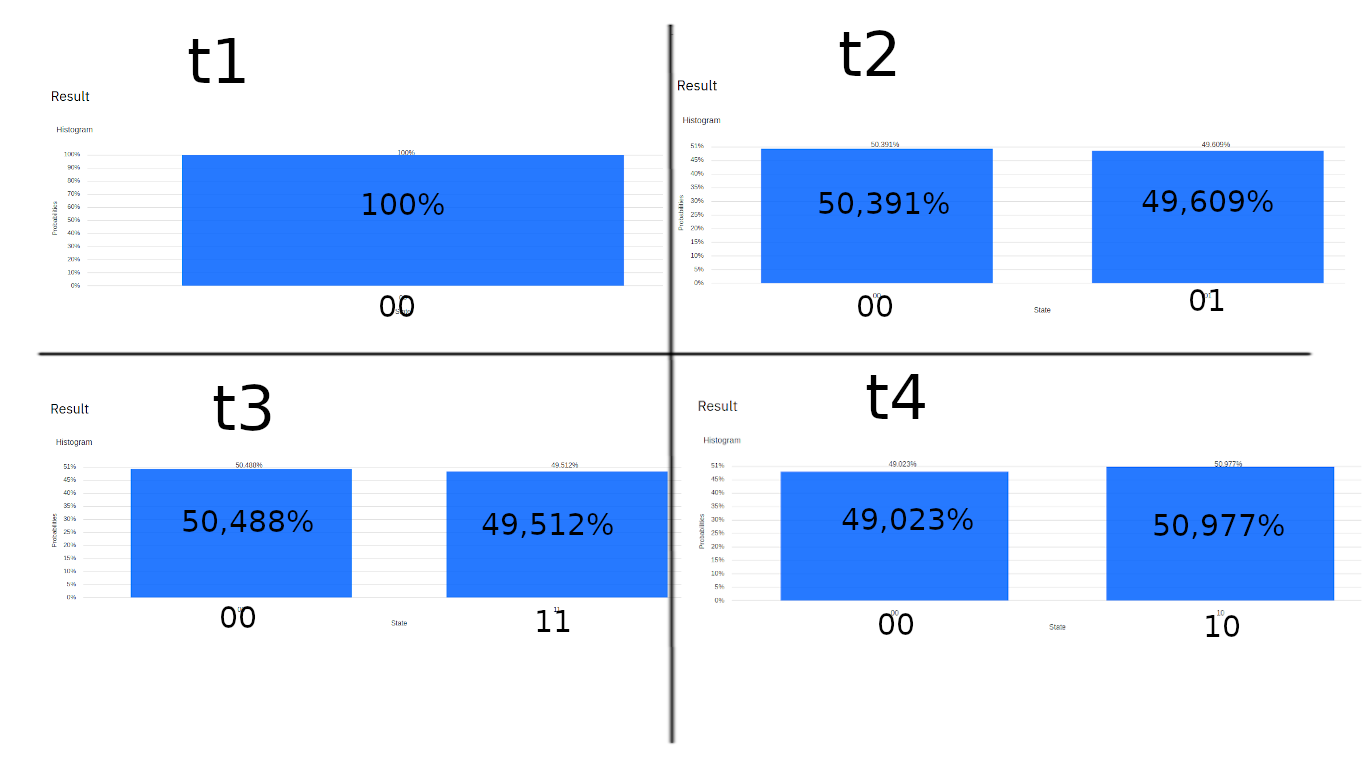
\includegraphics[width=.8\textwidth]{figures/expr1_qx_results.png} 
	\caption{Výsledky experimentu 1 z Quantum Experience so zvýraznenými 
údajmi.}

    \label{expr1_qx_results}
\end{figure}

Porovnajme naše výsledky so simulátorom IBM Quantum Experience. V IBM QX
bolo nutné vykonať štyri experimenty s rôznim časom merania, nakoľko tento
simulátor nepodporuje fiktívne meranie. Dosiahnuté výsledky sú na obrázku
\ref{expr1_qx_results}. Pripomeňme, že notácia dosiahnutých stavov v IBM QX
je \(\psi_1\psi_0\), teda v opačnom poradí ako zápis v našej tabuľke. V 
prvých dvoch merania sú výsledky totožné. Rozdiel nastáva pri prechode hradlom
\(CNOT\). Pravdepodobnostný model, ktorý využívame, funguje na istom 
matematickom aparáte. IBM QX je ale simulátor kantového počítača a teda môže 
brať do úvahy iné fyzikálne vlastnosti kvatových bitov, ktoré môžu vysvetľovať
rozdiel v našich výsledkoch.

\subsection{Experiment 2}
\begin{figure} 
	\centering 
	\includegraphics[width=.5\textwidth]{figures/expr2_circuit.png} 
	\caption{Obvod experimentu 2 s označenými časovými úsekmi meraní.}

    \label{expr2_circuit}
\end{figure}

Definujme kvantový obvod tak ako je na obrázku \ref{expr2_circuit}. Majme 
tri kvantové bity, ktoré označíme ako \(\psi_0\), \(\psi_1\) a \(\psi_2\).
Na prvých dvoch bitoch aktivujeme Hadamardové hradlá a potom tieto bity 
využijeme ako kontrólne bity v Tuffliho hradle. Nakoniec aplikujeme hradlo 
\(X\) a \(Z\).

V OpenQASM je tento obvod zostrojený ako
\begin{code}
qreg q[3];
creg c[3];

h q[0];
h q[1];
ccx q[0],q[1],q[2];
x q[0];
z q[1];
\end{code}

\subsection*{Teoretická analýza}
Stále platí, že
\[\ket{\psi_0} = \alpha_0\ket{0} + \beta_0\ket{1}\]
\[\ket{\psi_1} = \alpha_1\ket{0} + \beta_1\ket{1}\]
\[\ket{\psi_2} = \alpha_2\ket{0} + \beta_2\ket{1}\]
Zistiť stav systému v čase \(t_1\) je preto priamočiare
\[\ket{\psi} = \ket{\psi_0} \otimes \ket{\psi_1} \otimes \ket{\psi_2}\]

V čase \(t_2\) nastala aktivácia hradla \(H\) a preto sa zmení stav kvantových
bitov na 
\[\ket{\psi_0} = \frac{\alpha_0 + \beta_0}{\sqrt{2}}\ket{0} + \frac{\alpha_0 - \beta_0}{\sqrt{2}}\ket{1}\]
\[\ket{\psi_1} = \frac{\alpha_1 + \beta_1}{\sqrt{2}}\ket{0} + \frac{\alpha_1 - \beta_1}{\sqrt{2}}\ket{1}\]
\[\ket{\psi_2} = \alpha_2\ket{0} + \beta_2\ket{1}\]
Vyjadrenie pravdepodobností dosiahnutia stavov z meraní \(1\) a \(2\) sú 
zaznamenané v tabuľke \ref{expr2_tanal12}

\begin{table}
\centering
\begin{tabular}{|c|c|c|}
\hline
\textbf{Stav} & \multicolumn{2}{c|}{\textbf{Pravdepodobnosti}} \\
 & \(t_1\) & \(t_2\) \\
\hline
\(\ket{000}\) & \(|\alpha_0\alpha_1\alpha_2|^2\) & 
\(|\frac{\alpha_0 + \beta_0}{\sqrt{2}} \frac{\alpha_1 + \beta_1}{\sqrt{2}} \alpha_2|^2\) \\

\(\ket{001}\) & \(|\alpha_0\alpha_1\beta_2|^2\) & 
\(|\frac{\alpha_0 + \beta_0}{\sqrt{2}} \frac{\alpha_1 + \beta_1}{\sqrt{2}} \beta_2|^2\)  \\
%\hline

\(\ket{010}\) & \(|\alpha_0\beta_1\alpha_2|^2\) & 
\(|\frac{\alpha_0 + \beta_0}{\sqrt{2}} \frac{\alpha_1 - \beta_1}{\sqrt{2}} \alpha_2|^2\)   \\
%\hline

\(\ket{011}\) & \(|\alpha_0\beta_1\beta_2|^2\) &
\(|\frac{\alpha_0 + \beta_0}{\sqrt{2}} \frac{\alpha_1 - \beta_1}{\sqrt{2}} \beta_2|^2\)  \\
%\hline

\(\ket{100}\) & \(|\beta_0\alpha_1\alpha_2|^2\) &
\(|\frac{\alpha_0 - \beta_0}{\sqrt{2}} \frac{\alpha_1 + \beta_1}{\sqrt{2}} \alpha_2|^2\)   \\
%\hline

\(\ket{101}\) & \(|\beta_0\alpha_1\beta_2|^2\) &
\(|\frac{\alpha_0 - \beta_0}{\sqrt{2}} \frac{\alpha_1 + \beta_1}{\sqrt{2}} \beta_2|^2\)   \\
%\hline

\(\ket{110}\) & \(|\beta_0\beta_1\alpha_2|^2\) & 
 \(|\frac{\alpha_0 - \beta_0}{\sqrt{2}} \frac{\alpha_1 - \beta_1}{\sqrt{2}} \alpha_2|^2\)  \\
%\hline

\(\ket{111}\) & \(|\beta_0\beta_1\beta_2|^2\) & 
\(|\frac{\alpha_0 - \beta_0}{\sqrt{2}} \frac{\alpha_1 - \beta_1}{\sqrt{2}} \beta_2|^2\)   \\
\hline

\end{tabular}

\caption{\label{expr2_tanal12} Vyjadrenie meraní pravdepodobnosti v čase 
\(t_1\) a \(t_2\) experimentu 2.}
\end{table}


Časový okamih \(t_3\) predstavuje stav po prechode Tuffliho hradlom. Ak obe 
kontrólne bity \(\ket{\psi_0}\) a \(\ket{\psi_1}\) skolabujú do stavu 
\(\ket{1}\), tak cieľový bit \(\ket{\psi_2}\) bude preklopený hradlom \(X\).
Čiže v tomto momente \(\ket{\psi_0}\) kolabuje do \(\ket{1}\) s 
pravdepodobnosťou \(|\frac{\alpha_0 - \beta_0}{\sqrt{2}}|^2\) a podobne 
\(\ket{\psi_1}\) s pravdepodobnosťou \(|\frac{\alpha_1 - \beta_1}{\sqrt{2}}|^2\)
. Z toho vyplýva, že preklopenie bitu \(\ket{\psi_2}\) nastane
s pravdepodobnosťou  \(|\frac{\alpha_0 - \beta_0}{\sqrt{2}} \times \frac{\alpha_1 - \beta_1}{\sqrt{2}}|^2 = \frac{(\alpha_0 - \beta_0)^2(\alpha_1 - \beta_1)^2}{4}\)
\[\ket{\psi_2} = \beta_2\ket{0} + \alpha_2\ket{1}\]
Naopak s pravdepodobnosťou \(1 - \frac{(\alpha_0 - \beta_0)^2(\alpha_1 - \beta_1)^2}{4}\)
nenastane žiadna zmena
\[\ket{\psi_2} = \alpha_2\ket{0} + \beta_2\ket{1}\]

Toto rozdvojenie možných výsledkov sa nesie aj do merania \(t_4\), no zmena
nastáva len v prvých dvoch kvantových bitoch a tie sú v oboch prípadoch 
totožné. Nový stav týchto bitov teda je 
\[\ket{\psi_0} = \frac{\alpha_0 - \beta_0}{\sqrt{2}}\ket{0} + \frac{\alpha_0 + \beta_0}{\sqrt{2}}\ket{1}\]
\[\ket{\psi_1} = \frac{\alpha_1 + \beta_1}{\sqrt{2}}\ket{0} - \frac{\alpha_1 - \beta_1}{\sqrt{2}}\ket{1}\]

Merania \(t_3\) a \(t_4\) sú zaznamenané v tabuľke \ref{expr2_tanal34}.

\begin{table}
\centering
\begin{tabular}{|c|c|}
\hline
\textbf{Stav} & \textbf{Pravdepodobnosti} \\
 & \(t_3\) \\
\hline
\(\ket{000}\) &
\((|\frac{\alpha_0 + \beta_0}{\sqrt{2}} \frac{\alpha_1 + \beta_1}{\sqrt{2}} \beta_2|^2 \times P^{t3}_1) + (|\frac{\alpha_0 + \beta_0}{\sqrt{2}} \frac{\alpha_1 + \beta_1}{\sqrt{2}} \alpha_2|^2 \times P^{t3}_2)\)  \\
%\hline

\(\ket{001}\) & 
\((|\frac{\alpha_0 + \beta_0}{\sqrt{2}} \frac{\alpha_1 + \beta_1}{\sqrt{2}} \alpha_2|^2 \times P^{t3}_1) + (|\frac{\alpha_0 + \beta_0}{\sqrt{2}} \frac{\alpha_1 + \beta_1}{\sqrt{2}} \beta_2|^2 \times P^{t3}_2)\)  \\
%\hline

\(\ket{010}\) & 
\((|\frac{\alpha_0 + \beta_0}{\sqrt{2}} \frac{\alpha_1 - \beta_1}{\sqrt{2}} \beta_2|^2 \times P^{t3}_1) + (|\frac{\alpha_0 + \beta_0}{\sqrt{2}} \frac{\alpha_1 - \beta_1}{\sqrt{2}} \alpha_2|^2 \times P^{t3}_2)\)  \\
%\hline

\(\ket{011}\) & 
\((|\frac{\alpha_0 + \beta_0}{\sqrt{2}} \frac{\alpha_1 - \beta_1}{\sqrt{2}} \alpha_2|^2 \times P^{t3}_1) + (|\frac{\alpha_0 + \beta_0}{\sqrt{2}} \frac{\alpha_1 - \beta_1}{\sqrt{2}} \beta_2|^2 \times P^{t3}_2)\)  \\
%\hline

\(\ket{100}\) & 
\((|\frac{\alpha_0 - \beta_0}{\sqrt{2}} \frac{\alpha_1 + \beta_1}{\sqrt{2}} \beta_2|^2 \times P^{t3}_1) + (|\frac{\alpha_0 - \beta_0}{\sqrt{2}} \frac{\alpha_1 + \beta_1}{\sqrt{2}} \alpha_2|^2 \times P^{t3}_2)\)  \\
%\hline

\(\ket{101}\) & 
\((|\frac{\alpha_0 - \beta_0}{\sqrt{2}} \frac{\alpha_1 + \beta_1}{\sqrt{2}} \alpha_2|^2 \times P^{t3}_1) + (|\frac{\alpha_0 - \beta_0}{\sqrt{2}} \frac{\alpha_1 + \beta_1}{\sqrt{2}} \beta_2|^2 \times P^{t3}_2)\)  \\
%\hline

\(\ket{110}\) & 
\((|\frac{\alpha_0 - \beta_0}{\sqrt{2}} \frac{\alpha_1 - \beta_1}{\sqrt{2}} \beta_2|^2 \times P^{t3}_1) + (|\frac{\alpha_0 - \beta_0}{\sqrt{2}} \frac{\alpha_1 - \beta_1}{\sqrt{2}} \alpha_2|^2 \times P^{t3}_2)\)  \\
%\hline

\(\ket{111}\) & 
\((|\frac{\alpha_0 - \beta_0}{\sqrt{2}} \frac{\alpha_1 - \beta_1}{\sqrt{2}} \alpha_2|^2 \times P^{t3}_1) + (|\frac{\alpha_0 - \beta_0}{\sqrt{2}} \frac{\alpha_1 - \beta_1}{\sqrt{2}} \beta_2|^2 \times P^{t3}_2)\)  \\
\hline

 & \(t_4\) \\
\hline
\(\ket{000}\) &
\((|\frac{\alpha_0 - \beta_0}{\sqrt{2}} \frac{\alpha_1 + \beta_1}{\sqrt{2}} \beta_2|^2 \times P^{t3}_1) + (|\frac{\alpha_0 - \beta_0}{\sqrt{2}} \frac{\alpha_1 + \beta_1}{\sqrt{2}} \alpha_2|^2 \times P^{t3}_2)\)  \\
%\hline

\(\ket{001}\) & 
\((|\frac{\alpha_0 - \beta_0}{\sqrt{2}} \frac{\alpha_1 + \beta_1}{\sqrt{2}} \alpha_2|^2 \times P^{t3}_1) + (|\frac{\alpha_0 - \beta_0}{\sqrt{2}} \frac{\alpha_1 + \beta_1}{\sqrt{2}} \beta_2|^2 \times P^{t3}_2)\)  \\
%\hline

\(\ket{010}\) &
\((|\frac{\alpha_0 - \beta_0}{\sqrt{2}} \frac{\beta_1 - \alpha_1}{\sqrt{2}} \beta_2|^2 \times P^{t3}_1) + (|\frac{\alpha_0 - \beta_0}{\sqrt{2}} \frac{\beta_1 - \alpha_1}{\sqrt{2}} \alpha_2|^2 \times P^{t3}_2)\)  \\
%\hline

\(\ket{011}\) &
\((|\frac{\alpha_0 - \beta_0}{\sqrt{2}} \frac{\beta_1 - \alpha_1}{\sqrt{2}} \alpha_2|^2 \times P^{t3}_1) + (|\frac{\alpha_0 - \beta_0}{\sqrt{2}} \frac{\beta_1 - \alpha_1}{\sqrt{2}} \beta_2|^2 \times P^{t3}_2)\)  \\
%\hline

\(\ket{100}\) &
\((|\frac{\alpha_0 + \beta_0}{\sqrt{2}} \frac{\alpha_1 + \beta_1}{\sqrt{2}} \beta_2|^2 \times P^{t3}_1) + (|\frac{\alpha_0 + \beta_0}{\sqrt{2}} \frac{\alpha_1 + \beta_1}{\sqrt{2}} \alpha_2|^2 \times P^{t3}_2)\)  \\
%\hline

\(\ket{101}\) &
\((|\frac{\alpha_0 + \beta_0}{\sqrt{2}} \frac{\alpha_1 + \beta_1}{\sqrt{2}} \alpha_2|^2 \times P^{t3}_1) + (|\frac{\alpha_0 + \beta_0}{\sqrt{2}} \frac{\alpha_1 + \beta_1}{\sqrt{2}} \beta_2|^2 \times P^{t3}_2)\)  \\
%\hline

\(\ket{110}\) &
\((|\frac{\alpha_0 + \beta_0}{\sqrt{2}} \frac{\beta_1 - \alpha_1}{\sqrt{2}} \beta_2|^2 \times P^{t3}_1) + (|\frac{\alpha_0 + \beta_0}{\sqrt{2}} \frac{\beta_1 - \alpha_1}{\sqrt{2}} \alpha_2|^2 \times P^{t3}_2)\)  \\
%\hline

\(\ket{111}\) &
\((|\frac{\alpha_0 + \beta_0}{\sqrt{2}} \frac{\beta_1 - \alpha_1}{\sqrt{2}} \alpha_2|^2 \times P^{t3}_1) + (|\frac{\alpha_0 + \beta_0}{\sqrt{2}} \frac{\beta_1 - \alpha_1}{\sqrt{2}} \beta_2|^2 \times P^{t3}_2)\)  \\
\hline

\end{tabular}

\caption{\label{expr2_tanal34} Vyjadrenie meraní pravdepodobnosti v čase 
\(t_3\) a \(t_4\) experimentu 2, kde \(P^{t3}_1 = \frac{(\alpha_0 - \beta_0)^2(\alpha_1 - \beta_1)^2}{4}\) a \(P^{t3}_2 = 1 - \frac{(\alpha_0 - \beta_0)^2(\alpha_1 - \beta_1)^2}{4}\).}
\end{table}

\subsection*{Výpočet pravdepodobností pomocou pravdepodobnostného modelu}
Je nutné vyjadriť kvantový obvod v jazyku Haskell. Obvod obsahuje tri 
vertikálne levely. Pre meranie štyroch časových úsekov, ale definujeme 
štyri levely a štruktúry na ukladanie medzivýsledkov
\begin{code}
let l1 = Level [E, E, E] True
    l2 = Level [H, H, E] True
    l3 = Level [Cc, Cc, Ct] True
    l4 = Level [X, Z, E] True
    c = [l1, l2, l3, l4]
    st = StateTree 1 [q0, q0, q0] []
    rt = RT st []
\end{code}

Po spustení modelu sme dosiahli výsledky, ktoré sú zaznamenané v tabuľke
\ref{expr2_results}

\begin{table}
\centering
\begin{tabular}{|c|}
\hline
1.0 \\ 
000 \\ 
\hline
\end{tabular}

\begin{tabular}{|c|c|c|c|}
\hline
0.25 & 0.25 & 0.25 & 0.249 \\ 
000 & 010 & 100 & 110 \\ 
\hline
\end{tabular}

\begin{tabular}{|c|c|c|c|c|c|c|c|}
\hline
6.25e-2 & 6.249e-2 & 6.249e-2 & 6.249e-2 & 0.1875 & 0.1875 & 0.1875 & 0.18749 \\ 
001 & 011 & 101 & 111 & 000 & 010 & 100 & 110 \\ 
\hline
\end{tabular}

\begin{tabular}{|c|c|c|c|c|c|c|c|}
\hline
6.25e-2 & 6.249e-2 & 6.249e-2 & 6.249e-2 & 0.1875 & 0.1875 & 0.1875 & 0.18749 \\ 
001 & 011 & 101 & 111 & 000 & 010 & 100 & 110 \\ 
\hline
\end{tabular}

\caption{\label{expr2_results} Výsledky merania experimentu 2 pomocou
pravdepodobnostného modelu. Ohraničené riadky vymedzujú výsledky v jednotlivých
 časoch merania. Každá bunka obsahuje pravdepodobnosť dosiahnutia stavu a 
daný stav systému.}
\end{table}

Nakoľko na vstupe do systému sú kvantové bity v stave \(\ket{0}\) je jasné, že
meranie v čase \(t_1\) môže dosiahnúť len jediný výsledok, a to  \(000\).
V čase \(t_2\) sa vďaka Hadamardovému hradlu bity \(\ket{\psi_0}\) a 
\(\ket{\psi_1}\) dostanú do stavu \(\ket{+}\) a teda obe môžu s \(50\%\)-tnou
šancou kolabovať do \(\ket{1}\) alebo \(\ket{0}\). Čomu naznačujú aj výsledky.
Pri prechode Tuffliho hradlom systém môže zmeniť stav len ak prvé dva bity sú 
v stave \(\ket{1}\), a to môže nastať s \(25\%\)-tnou pravdepodobnosťou. Teda
aj výsledky zohľadňujú to, že je oveľa nižšia šanca že bit \(\ket{\psi_2}\)
je v preklopenom stave \(\ket{1}\). Pri poslednom meraní sa pravdepodobnosti
nemenia nakoľko aplikáciou hradla \(X\) na stav \(\ket{+}\) nenastane žiadna
zmena a aplikáciou \(Z\) sa stav zmení na \(\ket{-}\), čo nemá vplyv na
výsledok.

\begin{figure} 
	\centering 
	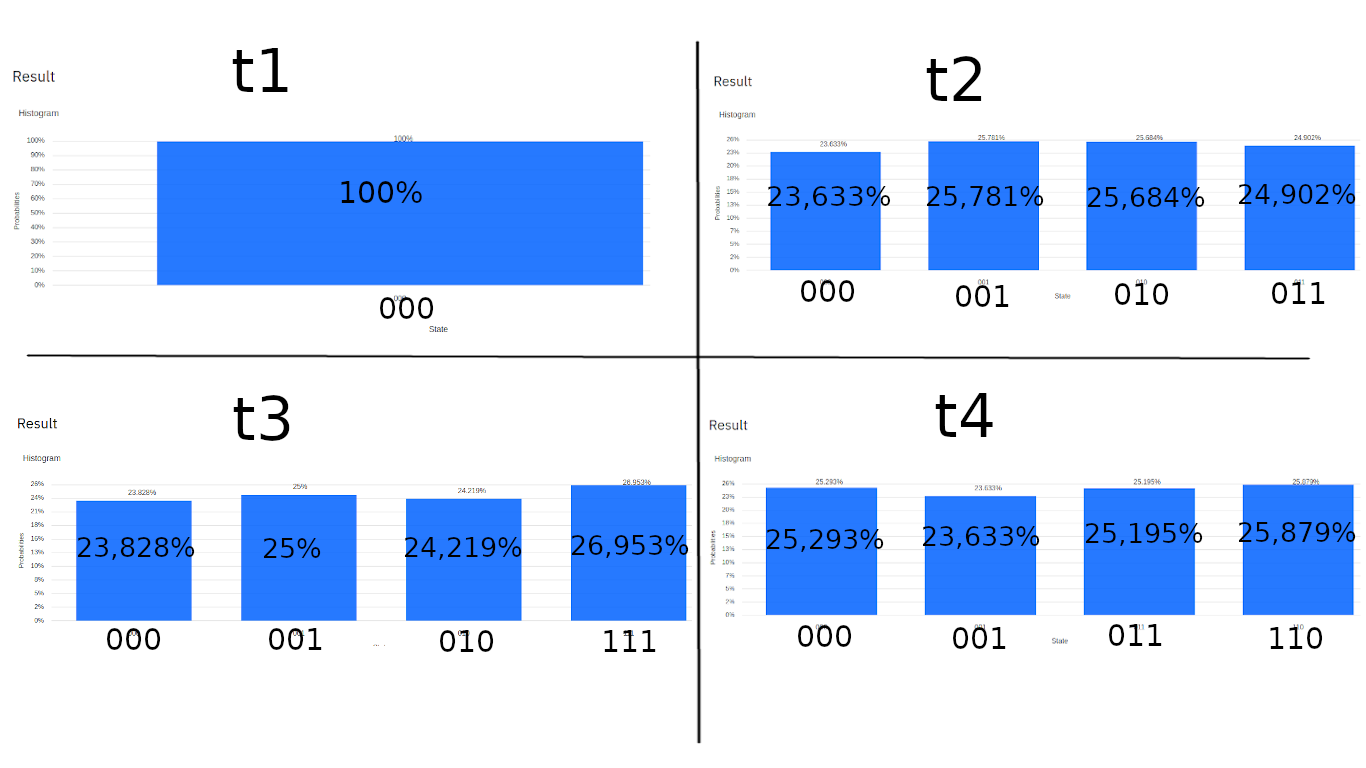
\includegraphics[width=.8\textwidth]{figures/expr2_qx_results.png} 
	\caption{Výsledky experimentu 2 z Quantum Experience so zvýraznenými 
údajmi.}

    \label{expr2_qx_results}
\end{figure}

Taktiež sme vykonali štyri merania v IBM QX, ktorých hodnoty sú zaznamenané
na obrázku \ref{expr2_qx_results}. Pripomeňme, že stav merania je zobrazovaný
v opačnom poradí ako v tabuľke \ref{expr2_results}. Teda kým u nás stav je 
v tvare \(c_0c_1c_2\), IBM QX využíva tvar \(c_2c_1c_0\). Ako sme očakávali, 
prvé dve merania skončili s výsledkom totožným s našim. Meranie v časoch 
\(t_3\) a \(t_4\) sa líšia. Predpokladom, pre rozdiel môže byť, že IBM QX 
využíva pri simulácii fyzikálny model nejakej častice, no náš pravdepodobnostný
model vychádza z matematickej reprezentácie kvantového bitu.

\subsection{Experiment 3}

\begin{figure} 
	\centering 
	\includegraphics[width=.6\textwidth]{figures/expr3_circuit.png} 
	\caption{Obvod experimentu 3 s označenými časovými úsekmi meraní.}
    \label{expr3_circuit}
\end{figure}

V treťom meraní použijeme ako hradlo \(CNOT\) aj \(CCNOT\). Na obrázku 
\ref{expr3_circuit} je zobrazený tento obvod. Nakoľko je známy stav systému
úplne na začiatku obvodu, tak tento časový úsek vynecháme a vykonáme opäť
štyri merania. Tento obvod je možné v IBM QX definovať pomocou OpenQASM 
nasledovne.
\begin{code}
qreg q[3];
creg c[3];

h q[0];
cx q[0],q[1];
h q[1];
ccx q[0],q[1],q[2];
\end{code}


\subsection*{Teoretická analýza}
Z obvodu je jasné, že v čase \(t_1\) zmena stavu nastane len pre bit 
\(\ket{\psi_0}\). A teda stavy budú nasledovné

\[\ket{\psi_0} = \frac{\alpha_0 + \beta_0}{\sqrt{2}}\ket{0} + \frac{\alpha_0 - \beta_0}{\sqrt{2}}\ket{1}\]
\[\ket{\psi_1} = \alpha_1\ket{0} + \beta_1\ket{1}\]
\[\ket{\psi_2} = \alpha_2\ket{0} + \beta_2\ket{1}\]

Odvodenie pravdepodobností je potom triviálne, 
\(\ket{\psi} = \ket{\psi_0} \otimes \ket{\psi_1} \otimes \ket{\psi_2}\).

Hradlo \(CNOT\) v čase \(t_2\) spôsobí vetvenie možných výsledkov. Čiže s 
pravdepodobnosťou \(P^{t2}_1 = \frac{(\alpha_0 + \beta_0)^2}{2}\) nadobudne
bit \(\ket{\psi_0}\) stav \(\ket{0}\), čo znamená, že \(\ket{\psi_1}\) ostane
nezmenené. Naopak s pravdepodobnosťou 
\(P^{t2}_2 = \frac{(\alpha_0 - \beta_0)^2}{2}\) nadobudne \(\ket{\psi_0}\) 
stav \(\ket{1}\), čo vedie k preklopeniu kvantového bitu \(\ket{\psi_1}\) na
\(X\ket{\psi_1}\).

Toto vetvenie sa takisto prenesie aj na meranie v čase \(t_3\). Takže 
aplikáciou Hadamardovho hradla na \(\ket{\psi_1}\) dostaneme
\begin{itemize}
    \item[] \(\ket{\psi_1} = \frac{\alpha_1 + \beta_1}{\sqrt{2}}\ket{0} + \frac{\alpha_1 - \beta_1}{\sqrt{2}}\ket{1}\) s pravdepodobnosťou  \(P^{t2}_1 = \frac{(\alpha_0 + \beta_0)^2}{2}\)

    \item[] \(\ket{\psi_1} = \frac{\beta_1 + \alpha_1}{\sqrt{2}}\ket{0} + \frac{\beta_1 - \alpha_1}{\sqrt{2}}\ket{1}\) s pravdepodobnosťou  \(P^{t2}_2 = \frac{(\alpha_0 - \beta_0)^2}{2}\)
\end{itemize} 

Znovupreviazaním kvantových bitov v obvode narastá počet počet možných stavov
geometricky. A teda v čase \(t_4\) už dostávame štyri možné výsledky s 
pravdepodobnosťami:
\begin{itemize}
    \item[] \(P^{t4}_1 = |\frac{\alpha_0 - \beta_0}{\sqrt{2}} \times \frac{\alpha_1 - \beta_1}{\sqrt{2}}|^2 \times P^{t2}_1 = \frac{(\alpha_0 - \beta_0)^2(\alpha_1-\beta_1)^2(\alpha_0+\beta_0)^2}{8}\)

    \item[] \(P^{t4}_2 = (1-|\frac{\alpha_0 - \beta_0}{\sqrt{2}} \times \frac{\alpha_1 - \beta_1}{\sqrt{2}}|^2) \times P^{t2}_1 = (1-\frac{(\alpha_0 - \beta_0)^2(\alpha_1-\beta_1)^2}{4}) \times \frac{(\alpha_0+\beta_0)^2}{2}\)

    \item[] \(P^{t4}_3 = |\frac{\alpha_0 - \beta_0}{\sqrt{2}} \times \frac{\beta_1 - \alpha_1}{\sqrt{2}}|^2 \times P^{t2}_2 = \frac{(\alpha_0 - \beta_0)^2(\beta_1-\alpha_1)^2(\alpha_0-\beta_0)^2}{8}\)

    \item[] \(P^{t4}_4 = (1-|\frac{\alpha_0 - \beta_0}{\sqrt{2}} \times \frac{\beta_1 - \alpha_1}{\sqrt{2}}|^2) \times P^{t2}_2 = (1-\frac{(\alpha_0 - \beta_0)^2(\beta_1-\alpha_1)^2}{4}) \times \frac{(\alpha_0-\beta_0)^2}{2}\)
\end{itemize}

Dajme do pozornosti, že \((\alpha_1 - \beta_1)^2 = (\beta_1 - \alpha_1)^2\),
teda ak označíme \(P_x = \frac{(\alpha_0 - \beta_0)^2(\alpha_1-\beta_1)^2}{4}\)
môžme pre tento experiment zapísať, že platí

\begin{itemize}
    \item[] \(P^{t4}_1 = P_x \times P^{t2}_1\)

    \item[] \(P^{t4}_2 = (1-P_x) \times P^{t2}_1\)

    \item[] \(P^{t4}_3 = P_x \times P^{t2}_2\)  

    \item[] \(P^{t4}_4 = (1-P_x) \times P^{t2}_2\)
\end{itemize}

V tabuľke \ref{expr3_t4_states} sú zapísané stavy kvantových bitov v čase
\(t_4\), pre všetky možné výsledky. Pre výpočet výsledných pravdepodobností
použijeme pre každú možnosť
\[\ket{\psi} = \ket{\psi_0} \otimes \ket{\psi_1} \otimes \ket{\psi_2}\]
Označme vyjadrenie pravdepodobnosti dosiahnutia nejakého celkového stavu 
ako \(P_{sn}\), kde \(1 \leq n \leq 4\) a \(s\) je stav. Potom platí
\[s = (P_{s1} \times P^{t4}_1) + (P_{s2} \times P^{t4}_2) + (P_{s3} \times P^{t4}_3) + (P_{s4} \times P^{t4}_4)\]

Čo vieme pomocou známych \(P^{t4}_n\) upraviť na 
\[s = (P_x \times P^{t2}_1)(P_{s1} - P_{s2} \times P^{t2}_1) + (P_x \times P^{t2}_2)(P_{s3} - P_{s4} \times P^{t2}_2) = \]
\[= (\frac{(\alpha^2_0 - \beta^2_0)(\alpha_1 - \beta_1)}{8})(P_{s1} - P_{s2} \times P^{t2}_1) + (\frac{(\alpha_0 - \beta_0)^2(\alpha_1 - \beta_2)^2}{8})(P_{s3} - P_{s4} \times P^{t2}_2) = \]
\[= \frac{(\alpha_1 - \beta_1)^2}{8}((\alpha^2_0 - \beta^2_0)(P_{s1} - P_{s2} \times \frac{(\alpha_0 + \beta_0)^2}{2})) + ((\alpha_0 - \beta_0)^2(P_{s3} - P_{s4} \times \frac{(\alpha_0 - \beta_0)^2}{2}))\]

Potom pre jednotlivé stavy sú dosiahnuteľné s pravdepodobnosťou
\begin{itemize}
\item[] \(\ket{000} = \frac{(\alpha_1 - \beta_1)^2}{8}((\alpha^2_0 - \beta^2_0)(\frac{(\alpha_0 + \beta_0)^2(\alpha_1 + \beta_1)^2}{4}\beta^2_2 - \frac{(\alpha_0 + \beta_0)^2(\alpha_1 + \beta_1)^2}{4}\alpha^2_2 \times \frac{(\alpha_0 + \beta_0)^2}{2})) + ((\alpha_0 - \beta_0)^2(\frac{(\alpha_0 + \beta_0)^2(\beta_1 + \alpha_1)^2}{4}\beta^2_2 - \frac{(\alpha_0 + \beta_0)^2(\beta_1 + \alpha_1)^2}{4}\alpha^2_2 \times \frac{(\alpha_0 - \beta_0)^2}{2}))\)

\item[] \(\ket{001} = \frac{(\alpha_1 - \beta_1)^2}{8}((\alpha^2_0 - \beta^2_0)(\frac{(\alpha_0 + \beta_0)^2(\alpha_1 + \beta_1)^2}{4}\alpha^2_2 - \frac{(\alpha_0 + \beta_0)^2(\alpha_1 + \beta_1)^2}{4}\beta^2_2 \times \frac{(\alpha_0 + \beta_0)^2}{2})) + ((\alpha_0 - \beta_0)^2(\frac{(\alpha_0 + \beta_0)^2(\beta_1 + \alpha_1)^2}{4}\alpha^2_2 - \frac{(\alpha_0 + \beta_0)^2(\beta_1 + \alpha_1)^2}{4}\beta^2_2 \times \frac{(\alpha_0 - \beta_0)^2}{2}))\) 

\item[] \(\ket{010} = \frac{(\alpha_1 - \beta_1)^2}{8}((\alpha^2_0 - \beta^2_0)(\frac{(\alpha_0 + \beta_0)^2(\alpha_1 - \beta_1)^2}{4}\beta^2_2 - \frac{(\alpha_0 + \beta_0)^2(\alpha_1 - \beta_1)^2}{4}\alpha^2_2 \times \frac{(\alpha_0 + \beta_0)^2}{2})) + ((\alpha_0 - \beta_0)^2(\frac{(\alpha_0 + \beta_0)^2(\beta_1 - \alpha_1)^2}{4}\beta^2_2 - \frac{(\alpha_0 + \beta_0)^2(\beta_1 - \alpha_1)^2}{4}\alpha^2_2 \times \frac{(\alpha_0 - \beta_0)^2}{2}))\)

\item[] \(\ket{011} = \frac{(\alpha_1 - \beta_1)^2}{8}((\alpha^2_0 - \beta^2_0)(\frac{(\alpha_0 + \beta_0)^2(\alpha_1 - \beta_1)^2}{4}\alpha^2_2 - \frac{(\alpha_0 + \beta_0)^2(\alpha_1 - \beta_1)^2}{4}\beta^2_2 \times \frac{(\alpha_0 + \beta_0)^2}{2})) + ((\alpha_0 - \beta_0)^2(\frac{(\alpha_0 + \beta_0)^2(\beta_1 - \alpha_1)^2}{4}\alpha^2_2 - \frac{(\alpha_0 + \beta_0)^2(\beta_1 - \alpha_1)^2}{4}\beta^2_2 \times \frac{(\alpha_0 - \beta_0)^2}{2}))\)

\item[] \(\ket{100} = \frac{(\alpha_1 - \beta_1)^2}{8}((\alpha^2_0 - \beta^2_0)(\frac{(\alpha_0 - \beta_0)^2(\alpha_1 + \beta_1)^2}{4}\beta^2_2 - \frac{(\alpha_0 - \beta_0)^2(\alpha_1 + \beta_1)^2}{4}\alpha^2_2 \times \frac{(\alpha_0 + \beta_0)^2}{2})) + ((\alpha_0 - \beta_0)^2(\frac{(\alpha_0 - \beta_0)^2(\beta_1 + \alpha_1)^2}{4}\beta^2_2 - \frac{(\alpha_0 - \beta_0)^2(\beta_1 + \alpha_1)^2}{4}\alpha^2_2 \times \frac{(\alpha_0 - \beta_0)^2}{2}))\)

\item[] \(\ket{101} = \frac{(\alpha_1 - \beta_1)^2}{8}((\alpha^2_0 - \beta^2_0)(\frac{(\alpha_0 - \beta_0)^2(\alpha_1 + \beta_1)^2}{4}\alpha^2_2 - \frac{(\alpha_0 - \beta_0)^2(\alpha_1 + \beta_1)^2}{4}\beta^2_2 \times \frac{(\alpha_0 + \beta_0)^2}{2})) + ((\alpha_0 - \beta_0)^2(\frac{(\alpha_0 - \beta_0)^2(\beta_1 + \alpha_1)^2}{4}\alpha^2_2 - \frac{(\alpha_0 - \beta_0)^2(\beta_1 + \alpha_1)^2}{4}\beta^2_2 \times \frac{(\alpha_0 - \beta_0)^2}{2}))\)

\item[] \(\ket{110} = \frac{(\alpha_1 - \beta_1)^2}{8}((\alpha^2_0 - \beta^2_0)(\frac{(\alpha_0 - \beta_0)^2(\alpha_1 - \beta_1)^2}{4}\beta^2_2 - \frac{(\alpha_0 - \beta_0)^2(\alpha_1 - \beta_1)^2}{4}\alpha^2_2 \times \frac{(\alpha_0 + \beta_0)^2}{2})) + ((\alpha_0 - \beta_0)^2(\frac{(\alpha_0 - \beta_0)^2(\beta_1 - \alpha_1)^2}{4}\beta^2_2 - \frac{(\alpha_0 - \beta_0)^2(\beta_1 - \alpha_1)^2}{4}\alpha^2_2 \times \frac{(\alpha_0 - \beta_0)^2}{2}))\) 

\item[] \(\ket{111} = \frac{(\alpha_1 - \beta_1)^2}{8}((\alpha^2_0 - \beta^2_0)(\frac{(\alpha_0 - \beta_0)^2(\alpha_1 - \beta_1)^2}{4}\alpha^2_2 - \frac{(\alpha_0 - \beta_0)^2(\alpha_1 - \beta_1)^2}{4}\beta^2_2 \times \frac{(\alpha_0 + \beta_0)^2}{2})) + ((\alpha_0 - \beta_0)^2(\frac{(\alpha_0 - \beta_0)^2(\beta_1 - \alpha_1)^2}{4}\alpha^2_2 - \frac{(\alpha_0 - \beta_0)^2(\beta_1 - \alpha_1)^2}{4}\beta^2_2 \times \frac{(\alpha_0 - \beta_0)^2}{2}))\) 

\end{itemize}

\begin{table}
\centering
\begin{tabular}{|l|c|}
\hline
\textbf{Pravdepodobnosť} & \textbf{Stavy \(\ket{\psi_0}\), \(\ket{\psi_1}\) a \(\ket{\psi_2}\)} \\
\hline
\(P^{t4}_1 = P_x \times P^{t2}_1\) & 
\(\ket{\psi_0} = \frac{\alpha_0 + \beta_0}{\sqrt{2}}\ket{0} + \frac{\alpha_0 - \beta_0}{\sqrt{2}}\ket{1}\) \\
& \(\ket{\psi_1} = \frac{\alpha_1 + \beta_1}{\sqrt{2}}\ket{0} + \frac{\alpha_1 - \beta_1}{\sqrt{2}}\ket{1}\) \\
& \(\ket{\psi_2} = \beta_2\ket{0} + \alpha_2\ket{1}\) \\
\hline

\(P^{t4}_2 = (1-P_x) \times P^{t2}_1\) & 
\(\ket{\psi_0} = \frac{\alpha_0 + \beta_0}{\sqrt{2}}\ket{0} + \frac{\alpha_0 - \beta_0}{\sqrt{2}}\ket{1}\) \\
& \(\ket{\psi_1} = \frac{\alpha_1 + \beta_1}{\sqrt{2}}\ket{0} + \frac{\alpha_1 - \beta_1}{\sqrt{2}}\ket{1}\) \\
& \(\ket{\psi_2} = \alpha_2\ket{0} + \beta_2\ket{1}\) \\
\hline

\(P^{t4}_3 = P_x \times P^{t2}_2\) & 
\(\ket{\psi_0} = \frac{\alpha_0 + \beta_0}{\sqrt{2}}\ket{0} + \frac{\alpha_0 - \beta_0}{\sqrt{2}}\ket{1}\) \\
& \(\ket{\psi_1} = \frac{\beta_1 + \alpha_1}{\sqrt{2}}\ket{0} + \frac{\beta_1 - \alpha_1}{\sqrt{2}}\ket{1}\) \\
& \(\ket{\psi_2} = \beta_2\ket{0} + \alpha_2\ket{1}\) \\
\hline

\(P^{t4}_4 = (1-P_x) \times P^{t2}_2\) & 
\(\ket{\psi_0} = \frac{\alpha_0 + \beta_0}{\sqrt{2}}\ket{0} + \frac{\alpha_0 - \beta_0}{\sqrt{2}}\ket{1}\) \\
& \(\ket{\psi_1} = \frac{\beta_1 + \alpha_1}{\sqrt{2}}\ket{0} + \frac{\beta_1 - \alpha_1}{\sqrt{2}}\ket{1}\) \\
& \(\ket{\psi_2} = \alpha_2\ket{0} + \beta_2\ket{1}\) \\
\hline
\end{tabular}

\caption{\label{expr3_t4_states} Tabuľka stavov kvantových bitov a
 pravdepodobností
nastatia týchto stavov v čase \(t_4\) experimentu 3.}
\end{table}

\subsection*{Výpočet pravdepodobností pomocou pravdepodobnostného modelu}
Definujme kvantový obvod pre pravdepodobnostný model.

\begin{code}
let l1 = Level [H, E, E] True
    l2 = Level [Cc, Ct, E] True
    l3 = Level [E, H, E] True
    l4 = Level [Cc, Cc, Ct] True
    c = [l1, l2, l3, l4]
    st = StateTree 1 [q0, q0, q0] []
    rt = RT st []
\end{code}

Za povšimnutie stojí fakt, že hradlá \(CNOT\) a \(CCNOT\) sú implementované
pomocou jednej funkcie. Takže aj v definícií obvodu nie je nutná špeciálna 
štruktúra pre zabezpečenie týchto hradiel, ale kontrólne bity sú jednoducho
označené ako \(Cc\) a cieľový bit ako \(Ct\).

Po spustení pravdepodobnostného modelu dostávame tabuľku s výsledkami 
\ref{expr3_results}

\begin{table}
\centering

\begin{tabular}{|c|c|}
\hline
0.50 & 0.49 \\ 
000 & 100 \\ 
\hline
\end{tabular}

\begin{tabular}{|c|c|c|c|}
\hline
0.25 & 0.249 & 0.250 & 0.25 \\ 
010 & 110 & 000 & 100 \\ 
\hline
\end{tabular}

\begin{tabular}{|c|c|c|c|c|c|c|c|}
\hline
0.125 & 0.1249 & 0.1249 & 0.1249 & 0.125 & 0.125 & 0.125 & 0.1249 \\ 
000 & 010 & 100 & 110 & 000 & 010 & 100 & 110 \\ 
\hline
\end{tabular}

\begin{tabular}{|c|c|c|c|c|c|c|c|}
\hline
3.1249e-2 & 3.1249e-2 & 3.1249e-2 & 3.1249e-2 & 9.375e-2 & 9.3749e-2 & 9.3749e-2 & 9.3749e-2  \\ 
001 & 011 & 101 & 111 & 000 & 010 & 100 & 110  \\ 

& & & & & & & \\

3.1251e-2 & 3.1249e-2 & 3.1249e-2 & 3.1249e-2 & 9.375e-2 & 9.3754e-2 & 9.3754e-2 & 9.375e-2 \\
001 & 011 & 101 & 111 & 000 & 010 & 100 & 110 \\
\hline
\end{tabular}

\caption{\label{expr3_results} Výsledky merania experimentu 3 pomocou
pravdepodobnostného modelu. Ohraničené riadky vymedzujú výsledky v jednotlivých
 časoch merania. Každá bunka obsahuje pravdepodobnosť dosiahnutia stavu a 
daný stav systému.}
\end{table}

Náš pravdepodobnostný model nesčítava pravdepodobnosti pri výskyte rovnakých 
stavov a automaticky sa meranie formátuje do jedného riadku. Z toho dôvodu sme 
naformátovali tabuľku tak aby boli všetky výsledky zobrazené.

Výsledky z IBM Quantum Experience sú zobrazené na obrázku \ref{expr3_qx_results}

\begin{figure} 
	\centering 
	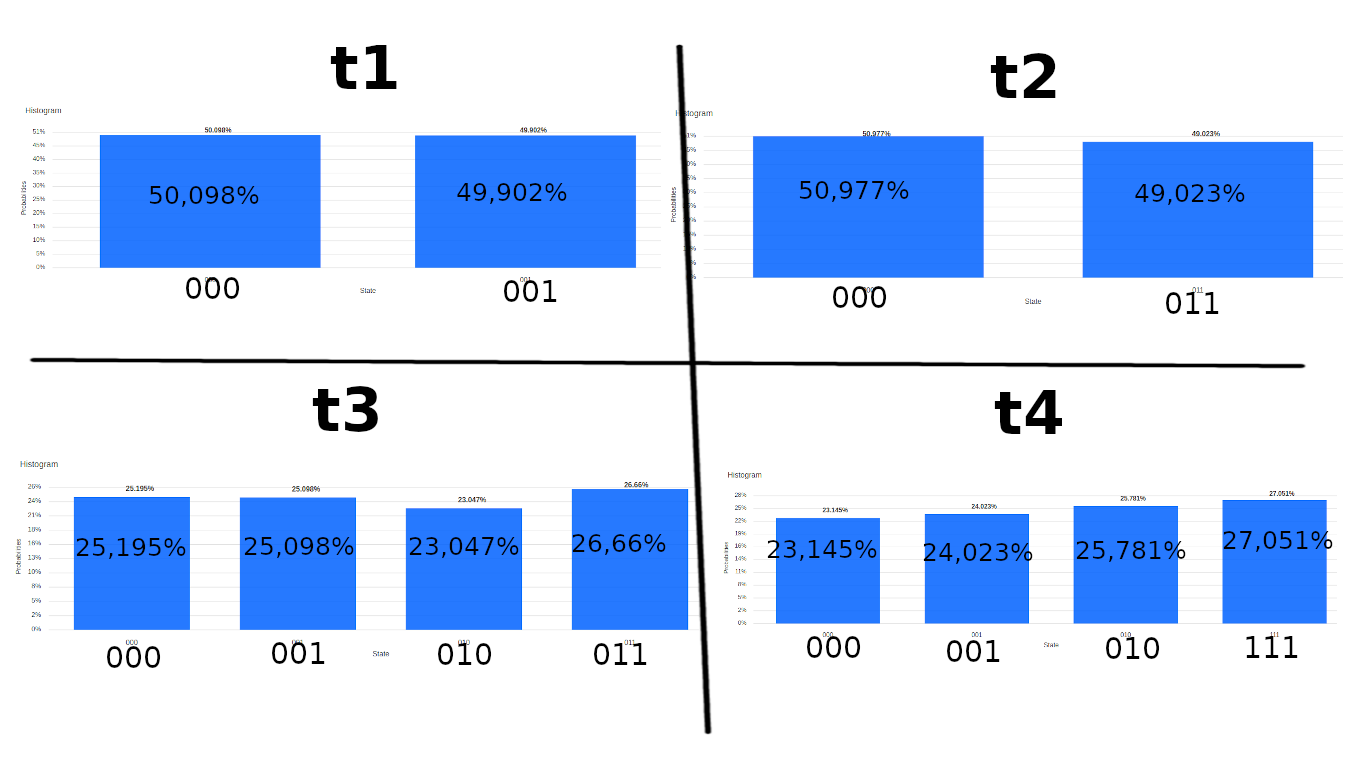
\includegraphics[width=.8\textwidth]{figures/expr3_qx_results.png} 
	\caption{Výsledky experimentu 3 z Quantum Experience so zvýraznenými 
údajmi.}

    \label{expr3_qx_results}
\end{figure}
